%
% Exemplo LaTeX de artigo UNISINOS
%
% Elaborado com base nas orientações dadas no documento
% ``GUIA PARA ELABORAÇÃO DE TRABALHOS ACADÊMICOS''
% disponível no site da biblioteca da Unisinos.
% http://www.unisinos.br/biblioteca
% 
% Os elementos textuais abaixo são apresentados na ordem em que devem
% aparecer no documento.  Repare que nem todos são obrigatórios - isso
% é devidamente indicado em cada caso.
%
% Comentários abaixo colocados entre aspas (`` '') foram
% extraídos diretamente do documento da biblioteca.
%
% Este documento é de domínio público.
%

%=======================================================================
% Declarações iniciais identificando a classe de documento e
% selecionando alguns pacotes adicionais.
%
% As opções disponíveis (separe-as com vírgulas, sem espaço) são:
% - twoside: Formata o documento para impressão frente-e-verso
%   (o default é somente-frente)
% - english,brazilian,french,german,etc.: idiomas usados no documento.
%   Deve ser colocado por último o idioma principal.
%=======================================================================
\documentclass[english,brazilian]{UNISINOSartigo} %twoside
\usepackage[utf8]{inputenc} % charset do texto (utf8, latin1, etc.)
\usepackage[T1]{fontenc} % encoding da fonte (afeta a sep. de sílabas)
\usepackage{graphicx} % comandos para gráficos e inclusão de figuras
\usepackage{bibentry} % para inserir refs. bib. no meio do texto
\usepackage{float}
\usepackage{array}
\usepackage{tabularx}
\usepackage{booktabs}
\usepackage{multirow}
\usepackage{newfloat}
\usepackage{setspace}
\usepackage{enumitem}
\usepackage{placeins}
%\usepackage{longtable}

\DeclareFloatingEnvironment[
fileext=loq,
listname={Lista de Quadros},
name=Quadro,
%placement=p,
%within=section,
%chapterlistsgaps=off
]{quadro}

\newcolumntype{L}{>{\centering\arraybackslash}m{6.2cm}}
\newcolumntype{G}{>{\centering\arraybackslash}m{5.5cm}}
\newcolumntype{A}{>{\centering\arraybackslash}m{2.4cm}}
\newcolumntype{B}{>{\centering\arraybackslash}m{7.5cm}}
%=======================================================================
% Escolha do sistema para geração de referências bibliográficas.
%
% O default é usar o estilo unisinos.bst.  Comente a definição abaixo
% e descomente a linha seguinte para usar o estilo do ABNTeX (é
% necessário ter esse pacote instalado).
%
% A vantagem do unisinos.bst é que ele permite o uso de um arquivo .bib
% seguindo as orientações tradicionais do BibTeX (veja essas orientações
% em http://ctan.tug.org/tex-archive/biblio/bibtex/contrib/doc/btxdoc.pdf).
% Entretanto, o estilo não suporta algumas citações mais exóticas como
% apud.  Para isso, use o ABNTeX, mas esteja ciente de que muitas de
% suas referências serão incompatíveis com os estilos tradicionais do
% BibTeX como plain, alpha, ieeetr, entre outros.
%=======================================================================
\usepackage[alf]{abntex2cite}

\autor{CLOSS FRAGA}{GUILHERME}
\titulo{Inteligência Artificial e \textit{Vibe Coding} no Processo de Desenvolvimento de \textit{Software}:}
\subtitulo{Um estudo comparativo entre desenvolvedores com e sem o uso de ferramentas de IA}
\orientador[Prof.ª Dra.]{Francisco}{Rosemary}
%\coorientador[Prof.~Dr.]{Lamport}{Leslie}
\local{São Leopoldo}
\ano{2025}
\unidade{Unidade Acadêmica de Graduação}
\curso{Curso de Bacharelado em Ciência da Computação}
\natureza{%
Artigo apresentado como requisito parcial para obtenção do título de Bacharel em Ciência da Computação, pelo Curso de Ciência da Computação da Universidade do Vale do Rio dos Sinos (UNISINOS)}

%=======================================================================
% Início do documento.
%=======================================================================

\begin{document}
\capa
\folhaderosto

% Diferentemente do normal, os comandos a seguir devem vir aqui mesmo,
% e não antes do \begin{document} onde seria o lugar deles. 
\tituloArtigo{Inteligência Artificial e \textit{Vibe Coding} no Processo de Desenvolvimento de \textit{Software}:}{Um estudo comparativo entre desenvolvedores com e sem o uso de ferramentas de IA}
\autorArtigo{Guilherme Closs Fraga\footnote{Graduando em Ciência da Computação pela Unisinos.  Email: guifraga8@edu.unisinos.br}}
\autorArtigo{Rosemary Francisco\footnote{Doutora em Administração. Email: rosemaryf@unisinos.br}}

%=======================================================================
% Resumo em Português.
%
% A recomendação é para 150 a 250 palavras.
%=======================================================================
\begin{abstract}
Lorem ipsum.

\palavraschave{lorem ipsum.}
\end{abstract}

\begin{otherlanguage}{english}
\singlespacing
\begin{abstract}
Lorem ipsum.
\end{abstract}
\palavraschave{lorem ipsum.}
\end{otherlanguage}

%=======================================================================
% Introdução
%=======================================================================
\section{Introdução}

A Inteligência Artificial (IA) é considerada uma das tecnologias mais transformadoras da atualidade, impulsionando mudanças em diversos setores e despertando interesse tanto no meio acadêmico quanto no mercado. Trata-se do uso de algoritmos e modelos computacionais capazes de realizar tarefas tradicionalmente dependentes da cognição humana, como análise de dados, raciocínio lógico e tomada de decisão (CÂNDIDO, 2022; AGUIAR, 2023). Segundo relatório da McKinsey (2025), a utilização de ferramentas de IA generativa pode aumentar a produtividade de desenvolvedores em tarefas de codificação, permitindo a execução de certas atividades até duas vezes mais rápido que processos totalmente manuais. Apesar desses avanços, a adoção dessas tecnologias levanta questões sobre dependência excessiva, erosão de habilidades humanas e confiabilidade das soluções geradas.

No contexto do desenvolvimento de \textit{software}, a presença da IA tem se tornado particularmente evidente. Ferramentas que combinam aprendizado de máquina e processamento de linguagem natural auxiliam desenvolvedores em diversas etapas do ciclo de vida do \textit{software}, desde a escrita de código até a detecção de falhas e a otimização de desempenho (COUTINHO et al., 2024). Um exemplo é o \textit{GitHub Copilot}, lançado em 2021 pela \textit{GitHub} em parceria com a \textit{OpenAI}, que utiliza modelos de IA Generativa (também chamadas de IA Gen) para sugerir trechos de código em tempo real \cite{github2021}. Da mesma forma, agentes de codificação baseados em IA, alinhados ao conceito de vibe coding, permitem que o desenvolvedor interaja de forma mais conversacional com a ferramenta, gerando código de maneira assistida, mas ainda mantendo controle sobre decisões críticas (CACM, 2025). Essas práticas têm sido discutidas como um avanço na programação assistida, trazendo benefícios de produtividade e colaboração entre humano e máquina.

Esses recursos, ao mesmo tempo em que oferecem praticidade e aumentam a produtividade, também levantam debates relevantes. Há questionamentos sobre até que ponto a utilização de IA generativa pode impactar o desenvolvimento de habilidades de raciocínio lógico e resolução de problemas, uma vez que o programador pode se tornar excessivamente dependente da ferramenta (VERASTEGUI; RUIZ; VILLANUEVA, 2025). Além disso, o código gerado pode apresentar erros lógicos, violações de boas práticas e vulnerabilidades de segurança, exigindo revisão crítica por parte do profissional (DEVOPS, 2024). Estudos experimentais indicam resultados variados: enquanto tarefas simples podem ser concluídas significativamente mais rápido com IA, contextos complexos podem exigir maior tempo de revisão e adaptação do código (PENG et al., 2023; METR, 2025).

Por outro lado, pesquisas recentes indicam que a adoção de IA no desenvolvimento de \textit{software} pode representar ganhos significativos em termos de produtividade e redução do tempo necessário para a entrega de soluções. Um estudo piloto com profissionais de \textit{software} demonstrou percepções majoritariamente positivas quanto ao impacto desses recursos na produtividade individual \cite{coutinho2024}. Essa realidade torna essencial a investigação de como essas ferramentas impactam o trabalho de desenvolvedores em contextos práticos. Assim, mais do que um recurso de conveniência, a IA se apresenta como um instrumento que pode redefinir processos e metodologias de engenharia de \textit{software}.

Diante desse cenário, torna-se essencial investigar como a IA generativa influencia o desempenho de desenvolvedores. Este trabalho propõe um estudo comparativo entre dois grupos de participantes: um com acesso a ferramentas de IA Generativa e outro sem acesso a esses recursos, aplicando um desafio técnico de programação. O objetivo é avaliar variáveis como eficiência, tempo de resolução e capacidade para solucionar os problemas propostos, fornecendo uma investigação sobre vantagens e limitações do uso dessas tecnologias.

Assim, o objetivo geral desta pesquisa é analisar o uso de ferramentas de IA Generativa no Desenvolvimento de \textit{Software} por meio de um desafio técnico comparativo entre desenvolvedores com e sem acesso a essas ferramentas. A questão de pesquisa que orienta este estudo é: de que maneira o uso de ferramentas de IA Generativa contribui ou afeta o desempenho de desenvolvedores em atividades práticas de programação? Espera-se que os resultados forneçam evidências consistentes para compreender o papel da IA como aliada no processo de desenvolvimento de \textit{software}, oferencedo resultados para pesquisadores, profissionais e instituições interessadas em compreender e orientar o uso dessas ferramentas emergentes.

\subsection{Objetivos Específicos}

Abaixo, destacam-se os objetivos específicos necessários para atingir a conclusão deste trabalho:
\begin{enumerate}[label=\alph*), leftmargin=1.2cm, itemsep=0.1em, topsep=0.1em]
    \item desenvolver uma plataforma \textit{web} simples para disponibilização do desafio técnico e coleta de dados de desempenho dos participantes;
    \item aplicar o desafio técnico a dois grupos de desenvolvedores, sendo um autorizado a utilizar ferramentas de IA e outro restrito ao uso dessas tecnologias;
    \item comparar os resultados obtidos pelos grupos em relação ao tempo de conclusão, qualidade do código entregue e abordagem adotada na resolução do problema;
    \item analisar as vantagens, limitações e possíveis implicações do uso de ferramentas de IA no processo de desenvolvimento de \textit{software}.
\end{enumerate}

\section{Fundamentação Teórica}

Com base na temática que o presente trabalho visa abordar, se faz necessário discorrer sobre dois tópicos fundamentais para a construção e consolidação do mesmo, sendo eles: Desenvolvimento de \textit{Software} e IA Generativa aplicada ao desenvolvimento de \textit{software}. Nas seções seguintes, os conceitos são explorados e detalhados a fim de estabelecer os fundamentos teóricos necessários para compor este trabalho.

\subsection{Desenvolvimento de \textit{Software}}

Um \textit{software} refere-se a todos os componentes não físicos de um computador, redes de computadores ou dispositivos móveis. Em linhas gerais, refere-se aos programas e aplicações, como o próprio sistema operacional, que fazem aquele aparelho (ou ferramenta) operar de acordo com o que o usuário necessita. Isto é, \textit{software} se trata de uma coleção de instruções, dados ou programas utilizados para operar computadores e executar determinadas tarefas \cite{coutinho2021}.

Em outras palavras, pode-se dizer que é um termo genérico que se refere à aplicações, \textit{scripts} e programas executáveis em um determinado dispositivo. Assim, o diferencia de \textit{hardware}, que descreve os aspectos físicos de um aparelho. Sendo assim, pode-se estabelecer o \textit{software} como um componente variável de um computador, enquanto o \textit{hardware} é constante \cite{sakurai2018}

De acordo com \citeonline{maynard2015}, existem basicamente dois tipos de \textit{software}, sendo eles: \textit{software} de aplicativo e \textit{software} de sistema. Um aplicativo seria aquele que atende uma necessidade específica ou executa determinadas tarefas. E, segundo \citeonline{schwab2019}, \textit{software} de sistema seria a parte essencial para que o \textit{hardware} de um computador opere, servindo como a plataforma para a execução de aplicativos. Ademais, pode-se mencionar outros tipos de \textit{software}, como os de programação, que são ferramentas necessárias para desenvolvedores, \textit{middlewares}, responsáveis por atuarem entre o \textit{software} do sistema e aplicativos e até mesmo \textit{drivers}, que são responsáveis por operarem dispositivos e periféricos de computadores.

Por fim, a sincronia entre diferentes tipos de \textit{software} e \textit{hardware}, é peça fundamental para o funcionamento eficiente de sistemas computacionais. Enquanto um aplicativo permite que seus usuários realizem determinadas tarefas, um sistema assegura que o \textit{hardware} opere corretamente, dando suporte para diferentes aplicações. Com a constante crescente de complexidade em sistemas modernos, a presença de um \textit{middleware} eficaz se torna indispensável para assegurar que diferentes \textit{softwares} funcionem em harmonia. Da mesma forma que, \textit{drivers} são indispensáveis para comunicação entre o sistema e periféricos, o que amplia as funcionalidades de um computador, resultando na melhoria da experiência do usuário.

Os \textit{softwares}, diferentemente do hardware, não são tangíveis e representam os componentes lógicos responsáveis pelo funcionamento de um computador ou dispositivo móvel. De acordo com \citeonline{candido2022}, o sistema operacional constitui o software fundamental, sendo exemplos mais conhecidos o \textit{Windows}, \textit{macOS} e \textit{Linux}, que variam em suas interfaces de usuário. Além dele, outros programas complementam as funções básicas, como o \textit{Microsoft Office} e o \textit{MediaPlayer} \cite{neto2019}, além de \textit{softwares} utilitários, como antivírus, ferramentas de \textit{backup} e manutenção de disco, que garantem desempenho e segurança. O avanço tecnológico também possibilitou o surgimento da virtualização, permitindo a execução de diferentes sistemas operacionais em uma única máquina física e ampliando a flexibilidade no uso dos recursos.

O \textit{software} pode ainda estar integrado diretamente ao \textit{hardware}, como em painéis eletrônicos de automóveis ou leitores de \textit{Blu-Ray}, caracterizando os chamados “embutidos” \cite{coutinho2021}. Historicamente, \textit{software} e \textit{hardware} eram concebidos como uma única unidade, sendo o termo “\textit{software}” empregado pela primeira vez por John W. Tukey em 1958 \cite{maynard2015}. Somente vinte anos depois, o governo dos Estados Unidos determinou que a IBM passasse a contabilizar \textit{hardware} e \textit{software} separadamente, o que abriu espaço para empresas especializadas \cite{sakurai2018}. Essa dissociação entre \textit{hardware} e \textit{software} impulsionou a inovação, permitindo atualizações independentes, acelerando ciclos de desenvolvimento e fomentando novos modelos de negócio baseados em \textit{software}, que hoje ocupam posição central na economia digital.

\citeonline{schwab2019} destaca que o trabalho do programador consiste, de forma essencial, em traduzir requisitos e algoritmos para uma linguagem de programação que o computador consiga interpretar e executar. A partir desse processo, é possível desenvolver diferentes tipos de \textit{software}, como aplicativos, jogos e sistemas de controle para robôs. Um exemplo histórico ligado à ideia de programação foi a invenção de um \textit{tear} “programável” pelo francês Joseph-Marie Jacquard, que representou um marco na Revolução Industrial. O equipamento não possuía processador, sendo controlado por meio de cartões perfurados. Conforme explica \citeonline{maynard2015}, esses cartões não utilizavam valores binários como 0 e 1, mas funcionavam através da presença ou ausência de perfurações: um furo indicava uma ação de movimento, enquanto a ausência significava outra. A criação de Jacquard é considerada uma das precursoras da automação moderna.

\citeonline{maynard2015} aponta que, em 1843, Augusta Ada King-Noel, mais conhecida como Ada Lovelace, desempenhou um papel marcante ao colaborar com Charles Babbage no projeto do \textit{Analytical Engine}, uma calculadora mecânica de uso geral que acabou não sendo concluída. Durante esse processo, Ada elaborou diversas anotações e descreveu um método para calcular os números de Bernoulli por meio da máquina, o que, segundo \citeonline{coutinho2021}, é considerado o primeiro programa de computador da história. Posteriormente, em 1941, Konrad Ernst Otto Zuse desenvolveu o Z3, reconhecido como o primeiro sistema de computação totalmente automatizado e programável do mundo.

O Z3 foi construído a partir dos conceitos idealizados por Babbage e tinha como diferencial a capacidade de realizar operações, como a adição, em menos de um quarto de segundo. O propósito central de sua criação estava ligado à busca por maior eficiência nos cálculos. Nos primeiros anos, os \textit{softwares} eram desenvolvidos para máquinas específicas e eram comercializados em conjunto com o \textit{hardware}. Já na década de 1980, passaram a ser distribuídos em mídias físicas, como disquetes, e mais tarde em CDs e DVDs. Atualmente, grande parte dos \textit{softwares} é obtida por meio da \textit{Internet}, seja diretamente nos sites dos fabricantes ou através de plataformas de distribuição de aplicativos.

Os modelos de ciclo de vida de \textit{software} descrevem as etapas que um sistema percorre desde sua concepção até sua desativação, organizando a sequência de atividades necessárias para o desenvolvimento. O objetivo central desses modelos é garantir qualidade, reduzir custos e otimizar o tempo de entrega. Entre as fases mais comuns estão:

\begin{itemize}[leftmargin=1cm, itemsep=0.1em, topsep=0.1em]
    \item Análise de Requisitos: onde são levantadas e documentadas as necessidades do sistema;
    \item Design: define a arquitetura, fluxos de trabalho e tecnologias a serem utilizadas;
    \item Implementação: fase em que o código é desenvolvido com base no planejamento estabelecido;
    \item Testes: que envolvem diferentes tipos de verificação para assegurar a confiabilidade do \textit{software};
    \item Manutenção: responsável por corrigir falhas e implementar melhorias após a entrega do sistema. 
\end{itemize}

De acordo com \citeonline{candido2022}, observa-se nos últimos anos uma tendência de desprofissionalização no aprendizado de programação, já que muitas pessoas têm adquirido essas habilidades de forma autodidata, recorrendo a tutoriais \textit{online} em vez de cursos formais. Além disso, o \textit{networking} global, aliado às diversas plataformas digitais, tem favorecido a formação de grandes comunidades que reúnem tanto entusiastas quanto programadores experientes, tornando cada vez menos nítida a distinção entre esses grupos.

Ao mesmo tempo, percebe-se um avanço significativo nos padrões e na qualidade do desenvolvimento de \textit{software}. Os sistemas estão cada vez mais sofisticados e complexos, o que aumenta a demanda por soluções digitais. Esse contexto reflete uma sociedade em constante transformação, onde as necessidades mudam rapidamente, gerando uma procura crescente por Desenvolvedores \textit{Full Stack} (um profissional de tecnologia que possui a capacidade de trabalhar em todas as camadas de um projeto de \textit{software}) em detrimento de profissionais especializados apenas em uma área.

A complexidade crescente dos sistemas requer profissionais capazes de atuar em todas as camadas do desenvolvimento, abrangendo desde o \textit{Frontend} (interface do usuário) até o \textit{Backend} (servidor, banco de dados e lógica de negócios de uma aplicação). Nesse cenário, os Desenvolvedores \textit{Full Stack} ganham destaque por sua flexibilidade e capacidade de adaptação às mudanças do mercado e às demandas dos usuários. Sua habilidade em compreender e integrar diferentes componentes de um sistema favorece um desenvolvimento mais unificado e eficiente, além de melhorar a comunicação e colaboração dentro das equipes. Assim, em um ambiente em que a agilidade e a adaptabilidade são fatores essenciais, esses profissionais se consolidam como recursos estratégicos para empresas que buscam manter a competitividade.

O desenvolvimento de \textit{software} pode ser entendido como um conjunto de atividades voltadas ao projeto, criação, implementação e manutenção de programas que orientam o funcionamento de computadores, sendo independente do \textit{hardware} e responsável por torná-los programáveis \cite{schwab2019}.

Conforme aponta \citeonline{candido2022}, o desenvolvimento de \textit{software} deve ser integrado ao desenvolvimento de produtos mecânicos e elétricos, o que faz com que o papel dos desenvolvedores de \textit{software} seja menos delimitado em comparação ao dos engenheiros. Esses profissionais podem focar em áreas específicas do projeto, como a codificação, enquanto o ciclo de vida do \textit{software} envolve a transformação de requisitos em funcionalidades, o trabalho em equipes multifuncionais, a gestão de processos e equipes, além de atividades de teste e manutenção.

De acordo com \citeonline{schwab2019}, a atuação dos desenvolvedores de \textit{software} vai além das equipes de programação, envolvendo também cientistas e fabricantes de dispositivos e \textit{hardware}, que contribuem para a criação de códigos, mesmo não sendo os principais responsáveis pelo desenvolvimento. Essa participação não se limita às indústrias tradicionais de tecnologia da informação, abrangendo também empresas que não se dedicam exclusivamente à produção de \textit{software} ou semicondutores.

A ampliação do papel dos desenvolvedores de \textit{software} evidencia a crescente integração da tecnologia da informação com diversas áreas, como ciência, medicina, engenharia e artes. Atualmente, o desenvolvimento de \textit{software} é fundamental para múltiplos setores, desde a indústria automotiva até o entretenimento, impulsionando a inovação e a transformação digital. Na indústria automotiva, esses profissionais são essenciais para o desenvolvimento de sistemas de condução autônoma e tecnologias avançadas de segurança. Já no cinema, os efeitos visuais e a animação digital dependem fortemente do \textit{software} para criar mundos e personagens realistas. Dessa forma, os desenvolvedores de \textit{software} exercem um papel cada vez mais diversificado e influente, moldando o futuro em diferentes áreas do conhecimento e da atividade humana.

\subsubsection{Modelos de Desenvolvimento de \textit{Software}}

O desenvolvimento de \textit{software} pode ser conduzido por diferentes abordagens, conhecidas como modelos de processo de \textit{software}. Esses modelos têm como objetivo estruturar e organizar as atividades necessárias para transformar requisitos em um produto final de qualidade. Existem diversos modelos conhecidos, mas para fins de exemplificar os dois mais conhecidos, podemos citar o Modelo Cascata e os Modelos Ágeis.

O Modelo Cascata (ou \textit{Waterfall}) foi um dos primeiros modelos formais de processo de software. Proposto por Winston Royce em 1970, consiste em uma sequência linear de fases: levantamento de requisitos, análise, projeto, implementação, testes, implantação e manutenção. Cada fase deve ser concluída antes do início da próxima, funcionando como uma “cascata” de atividades \cite{sommerville2011}. Entre suas vantagens podemos citar:

\begin{itemize}[leftmargin=1cm, itemsep=0.1em, topsep=0.1em]
    \item Estrutura simples e de fácil entendimento;
    \item Definição clara das fases e entregas;
    \item Útil em projetos com requisitos bem definidos e estáveis.
\end{itemize}

Por outro lado, há também desvantagens que valem ser destacadas deste modelo, sendo elas:

\begin{itemize}[leftmargin=1cm, itemsep=0.1em, topsep=0.1em]
    \item Pouca flexibilidade diante de mudanças nos requisitos;
    \item Risco de identificação tardia de falhas, geralmente apenas na fase de testes;
    \item Dificuldade em lidar com projetos complexos ou inovadores.
\end{itemize}

Os Modelos Ágeis surgiram como uma alternativa aos modelos tradicionais, sendo formalizados em 2001 com o Manifesto Ágil. Esses modelos priorizam colaboração com o cliente, entregas rápidas e contínuas, adaptação às mudanças e interações entre pessoas mais do que processos rígidos \cite{beck2001}.

Entre os métodos ágeis mais utilizados, principalmente nos dias atuais, estão o \textit{Scrum}, o \textit{Kanban} e o \textit{Extreme Programming} (conhecido também como \textit{XP}). Todos eles seguem o princípio de dividir o projeto em pequenos ciclos (iterações), resultando em entregas frequentes e incrementais do produto. Como as principais vantagens, podemos citar:

\begin{itemize}[leftmargin=1cm, itemsep=0.1em, topsep=0.1em]
    \item Alta flexibilidade para mudanças de requisitos;
    \item Entregas rápidas que geram valor contínuo ao cliente;
    \item Melhora na comunicação e na colaboração entre equipe e \textit{stakeholders}.
\end{itemize}

E, das suas principais desvantagens:

\begin{itemize}[leftmargin=1cm, itemsep=0.1em, topsep=0.1em]
    \item Pode gerar falta de documentação formal, dependendo da equipe;
    \item Requer alto envolvimento do cliente no processo;
    \item Menos indicado para projetos de missão crítica que demandam forte rastreabilidade.
\end{itemize}

Sendo assim, evidencia-se que cada modelo de desenvolvimento possui suas características, vantagens e limitações. A escolha do modelo mais adequado depende do contexto do projeto, da complexidade do sistema, do nível de risco, do grau de inovação e da estabilidade dos requisitos. Modelos tradicionais como Cascata são mais estruturados, os modelos Ágeis oferecem maior flexibilidade e adaptabilidade, características cada vez mais valorizadas no mercado atual. Na Tabela \ref{tab:modelosDev}, temos um comparativo resumido dos principais pontos dos modelos citados.

\begin{table}[ht]
    \caption{Comparativo entre Modelo Cascata e Modelos Ágeis}
    \label{tab:modelosDev}
    \centering%
    \footnotesize
    \begin{tabularx}{\textwidth}{lXXXX}
        \toprule
        \textbf{Modelo} & \textbf{Resumo} & \textbf{Vantagem} & \textbf{Desvantagem} & \textbf{Indicado para}\\
        \midrule
        Cascata & Linear e sequencial & Simples e claro & Pouca flexibilidade & Projetos pequenos e estáveis \\
        \midrule
        Ágeis & Iterativo e adaptável & Entregas rápidas & Pouca documentação & Projetos dinâmicos e mutáveis \\
        \bottomrule
    \end{tabularx}
    \fonte{Elaborado pelo autor}
\end{table}
\FloatBarrier

\subsection{IA Generativa (aplicada ao desenvolvimento de \textit{software})}

A Inteligência Artificial (IA) consolidou-se como uma das áreas mais relevantes da Ciência da Computação, devido à sua capacidade de simular processos cognitivos humanos como aprendizagem, raciocínio e tomada de decisão por meio de algoritmos e modelos matemáticos (CÂNDIDO, 2022; AGUIAR, 2023). Nos últimos anos, a evolução tecnológica permitiu que esses sistemas ultrapassassem o campo do reconhecimento de padrões e da automação, alcançando um estágio em que são capazes de gerar novos conteúdos, fenômeno que deu origem ao conceito de Inteligência Artificial Generativa. Segundo Uniphore (2024), a IA Generativa refere-se ao ramo da IA que cria resultados originais — textos, imagens, sons ou códigos — a partir de grandes volumes de dados já existentes, distinguindo-se de modelos meramente classificatórios ou preditivos. Conforme aponta TechTarget (2024), esse processo ocorre por meio da análise de padrões e estruturas aprendidas, sendo ativado a partir de instruções em linguagem natural, conhecidas como prompts.

No campo do desenvolvimento de software, a IA Generativa tem desempenhado papel crescente ao possibilitar a geração automática de trechos de código, documentação, testes e até refatoração de programas. Idrisov e Schlippe (2024) compararam códigos produzidos por ferramentas de IA e por programadores humanos, identificando que, embora as soluções geradas automaticamente sejam satisfatórias em tarefas de baixa complexidade, ainda apresentam limitações em contextos que exigem maior profundidade técnica ou conhecimento de domínio. Em estudo semelhante, Yu (2025) observou que assistentes de codificação generativa, como Codeium e ferramentas similares, aumentam a produtividade em atividades repetitivas, mas enfrentam dificuldades quando aplicados a tarefas que demandam compreensão arquitetural ou integração com sistemas legados.

Outro aspecto recorrente na literatura é a avaliação da qualidade do código gerado. Yetiştiren et al. (2023) realizaram um comparativo entre GitHub Copilot, Amazon CodeWhisperer e ChatGPT, utilizando o benchmark HumanEval. Os resultados apontaram variações significativas em critérios como correção, confiabilidade e manutenibilidade, indicando que tais ferramentas funcionam melhor como apoio ao programador do que como substitutos plenos. A segurança do software também se apresenta como desafio relevante: de acordo com Alwageed e Khan (2025), embora a IA Generativa possa contribuir para práticas de codificação segura, existe o risco de introdução de vulnerabilidades e de não conformidade com padrões regulatórios.

Por fim, é importante destacar as discussões éticas e sociais associadas ao uso da IA Generativa. Afreen, Mohaghegh e Doborjeh (2025) ressaltam que problemas como a contextualização insuficiente do código, a geração de erros sutis e as preocupações relacionadas a direitos autorais e privacidade ainda carecem de soluções adequadas. Nesse sentido, observa-se que a IA Generativa aplicada ao desenvolvimento de software apresenta grande potencial de aumento de produtividade e inovação, mas exige acompanhamento crítico, validações constantes e reflexões acerca de suas limitações e implicações sociais.

\section{Trabalhos Relacionados}

Para fins de melhor localizar os trabalhos com temáticas relacionadas para o presente estudo, foi utilizado a plataforma de busca especializada em literatura acadêmica e científica Google Scholar. Os procedimentos de pesquisa e seleção consistiram em utilizar palavras chaves em português como “inteligência artificial generativa”, “desenvolvimento de software”, “produtividade”, “suporte”, “otimização” e “performance”, variando também os termos em inglês. Por fim, para selecionar os trabalhos a seguir, foi considerado o contexto do estudo de cada autor, conceitos abordados, tecnologias mencionadas e/ou utilizadas e problemáticas ressaltadas, que melhor correlacionassem com o presente estudo.

\subsection{Trabalhos Acadêmicos}

Dado o contexto do aprimoramento e evolução de Inteligências Artificiais Generativas nos anos recentes, tal como suas aplicabilidades para otimização de tarefas voltadas para a área de desenvolvimento de software, diversos estudos têm sido realizados com o intuito de explorar ainda mais os conceitos técnicos e práticos. A seguir, são apresentados estudos e pesquisas relacionados ao tema, estabelecendo um paralelo com a temática abordada para este trabalho.

\citeonline{gomes2023} apresenta uma análise comparativa de diferentes Inteligências Artificiais Generativas (IAs Generativas) aplicadas no desenvolvimento de software, mas particularmente focando em ferramentas auxiliares como \textit{GitHub Copilot}, \textit{Codeium}, \textit{Tabnine} e \textit{CodeGeeX}. Para fins práticos, seu trabalho focou em experimentos utilizando \textit{GitHub Copilot} e \textit{Codeium} para mensurar a eficiência das ferramentas.

Como resultado, o \citeonline{gomes2023} aponta que ambas as tecnologias se mostram extremamente úteis no processo de otimização do desenvolvimento, produtividade e qualidade de códigos, com a escolha entre elas dependendo das necessidades particulares do projeto e das preferências do profissional. Entretanto, o destaque ficou para a ferramenta \textit{GitHub Copilot}, que apresentou uma leve vantagem, com uma capacidade superior de compreensão para construção de uma lógica de desenvolvimento mais coesa.

Em \citeonline{daSilva2025}, é realizado o teste prático de viabilidade de desenvolvimento de uma aplicação \textit{web} para gerenciamento de sócios torcedores de um clube de futebol, utilizando IA Generativa como apoio na construção da aplicação. Ainda que, neste estudo os autores desenvolveram uma solução simples, utilizando tecnologias como \textit{JavaScript}, \textit{PHP}, \textit{HTML5} e entre outras, o trabalho demonstrou que utilizar de Inteligência Artificial otimiza o processo de desenvolvimento, desde a geração de código, identificação de falhas e sugestões de melhores práticas para a construção de soluções.

De acordo com os autores e os resultados obtidos \cite{daSilva2025}, a adoção de IA Generativa no processo de desenvolvimento contribui tanto para acelerar a produção, quanto para a qualidade e otimização da aplicação. Para o estudo em questão, os autores contaram com o suporte de modelos de IA Generativa como \textit{GPT-3.5} e \textit{Claude 1}.

Em contrapartida, no trabalho de \citeonline{ferreira2023}, o autor aborda sobre a influência das IAs Generativas na área de desenvolvimento de software, com base em um estudo qualitativo, combinando cenários exploratórios e descritivos. Aqui, o autor menciona o uso de ferramentas como o \textit{ChatGPT}, \textit{Bard}, \textit{GitHub Copilot} para tratar sobre a temática de modelos baseados no conceito de Processamento de Linguagem Natural (PLN).

Ao longo de seu estudo, \citeonline{ferreira2023} aborda questões como o impacto da Inteligência Artificial na programação, trazendo dados e referências, para dissertar sobre tópicos como os desafios e benefícios do uso de ferramentas de IA. Sobre os desafios, o autor menciona a questão da dependência do uso de IA, limitando assim o desenvolvimento de habilidades próprias por parte do programador e a substituição do desenvolvedor por IA, assunto fortemente debatido desde a evolução das IAs Generativas nos anos recentes. 

\citeonline{santos2024} investigou a influência das ferramentas de IA Generativas, citando \textit{ChatGPT} e \textit{GitHub Copilot}, com foco no processo de ensino e aprendizagem das instituições de ensino superior na área de desenvolvimento de \textit{software}. O objetivo deste estudo consistiu em identificar oportunidades e desafios no uso destas tecnologias. Para isso, o autor realizou um comparativo com grupos de alunos iniciantes, estagiários no setor de tecnologia, alocando-os em um projeto simulado.

Para tanto o autor \cite{santos2024} seguiu um delineamento \textit{crossover} 2x2 AB/BA, isto é, alternando os grupos entre o uso e não uso de IA. Após a coleta de dados, foi mensurado o conhecimento técnico dos grupos, tal como qualidade dos artefatos gerados, avaliação do produto desenvolvido e provas simuladas para testar o conhecimento adquirido. Aqui, o autor ressalta que os grupos que fizeram o uso de IA obtiveram melhores avaliações nos artefatos desenvolvidos, desde a documentação ao desenvolvimento de \textit{software} propriamente dito. Entretanto, a nível de conhecimento, não refletiu em avaliações melhores nas provas simuladas (notas de avaliações, propriamente).

\citeonline{costa2024} explorou como o uso de IA Generativa pode otimizar e aprimorar o processo de desenvolvimento de \textit{software} no contexto empresarial. O autor conduziu uma extensa revisão bibliográfica com o intuito de identificar as ferramentas e metodologias mais atuais e eficazes no mercado. A partir de então, selecionou e implementou \textit{frameworks} como \textit{Spring Boot} para a construção de uma aplicação escalável em \textit{Java}, utilizando o \textit{ChatGPT} como ferramenta de suporte durante o processo.

Ademais, o autor \cite{costa2024} fez o uso de ferramentas de teste e documentação de \textit{APIs}, tais como \textit{Postman} e até mesmo \textit{JUnit}, como \textit{framework} para validação de testes unitários. Em seu trabalho, o autor utilizou a IA Generativa através de \textit{prompts} para criação de todos os requisitos, códigos e validações do seu projeto. Como resultado, ele evidenciou uma melhoria na eficiência tanto do desenvolvimento quanto da qualidade da aplicação entregue. Entretanto, ressaltou a importância de que, o conhecimento prévio para uso de IAs Generativas é fundamental, para que se torne possível o uso da mesma como ferramenta de apoio no processo de desenvolvimento de \textit{software}.

Por fim, com base nos estudos analisados e considerando o crescimento acelerado das ferramentas de Inteligência Artificial Generativa na atualidade, evidencia-se que o profissional — independentemente da área de atuação — pode, e deve, tirar proveito dessas tecnologias para se manter em constante aprendizado e adaptado às novas realidades do mercado. Ou seja, não é necessário dominar todos os princípios técnicos por trás dessas ferramentas, mas sim saber utilizá-las estrategicamente, visando otimização, desempenho e melhores resultados.

Dessa forma, a proposta deste estudo é analisar, com base em dados e indicadores, o quanto o uso da Inteligência Artificial Generativa pode contribuir, junto aos profissionais da área de desenvolvimento de \textit{software}, para a entrega de soluções mais ágeis. Para delimitar o foco principal do trabalho, o segmento analisado será o desenvolvimento de software, considerando o papel do desenvolvedor no cenário atual do mercado de trabalho.

Com base no levantamento de todas as informações dos trabalhos relacionados ao tema, é possível agrupar as principais características de cada um deles para fins de comparação. Dada as informações levantadas, separa-se as características em quatro parâmetros, sendo eles:

\begin{itemize}[leftmargin=1cm, itemsep=0.1em, topsep=0.1em]
    \item  \textbf{Tema principal:} define qual foi o principal tema abordado ao longo do estudo;
    \item \textbf{Metodologia aplicada:} define o modelo utilizado para o estudo em questão;
    \item \textbf{Tecnologias/Inteligências Artificiais utilizadas:} se aplicável, define as ferramentas e/ou tecnologias utilizadas para fins de estudo, tal como o modelo de Inteligência Artificial utilizado ou analisado;
    \item \textbf{Objetivo:} define o objetivo do modelo, ou seja, qual problemática o modelo buscou esclarecer ao seu decorrer.
\end{itemize}

A partir do resultado do levantamento de trabalhos relacionados, foi possível elaborar a Tabela \ref{tab:estudos}, onde mostra o conteúdo dos critérios apontados em cada estudo, por ordem de apresentação.

\begin{table}[ht]
    \caption{Comparativo entre os trabalhos relacionados}
    \label{tab:estudos}
    \centering%
    \footnotesize
    \begin{tabularx}{\textwidth}{lXXXX}
        \toprule
        \textbf{Autores} & \textbf{Tema} & \textbf{Metodologia} & \textbf{Tecnologias/IA} & \textbf{Objetivo}\\
        \midrule
        \citeonline{gomes2023} & Comparação de IAs no desenvolvimento de \textit{software} & Testes práticos comparativos & \textit{GitHub Copilot}, \textit{Codeium}, \textit{Tabnine}, \textit{CodeGeeX} & Avaliar eficiência de ferramentas de IA no desenvolvimento \\
        \midrule
        \citeonline{daSilva2025} & Aplicação de IA na criação de sistemas \textit{web} & Estudo de caso com experimento & \textit{JavaScript}, \textit{PHP}, \textit{HTML5}, \textit{GPT-3.5}, \textit{Claude 1} & Verificar ganho de produtividade com uso de IA \\
        \midrule
        \citeonline{ferreira2023} & Impacto da IA na programação & Estudo qualitativo exploratório & \textit{ChatGPT}, \textit{Bard}, \textit{GitHub Copilot} & Analisar benefícios e riscos do uso da IA \\
        \midrule
        \citeonline{santos2024} & IA no ensino de tecnologia & Experimento com grupos (\textit{crossover}) & \textit{ChatGPT}, \textit{GitHub Copilot} & Medir impacto da IA na aprendizagem e desempenho técnico \\
        \midrule
        \citeonline{costa2024} & Uso de IA Generativa no desenvolvimento de \textit{software} empresarial & Revisão bibliográfica com aplicação prática & \textit{Spring Boot}, \textit{Java}, \textit{ChatGPT}, \textit{Postman}, \textit{JUnit} & Otimizar e melhorar eficiência e qualidade no desenvolvimento de aplicações \\
        \bottomrule
    \end{tabularx}
    \fonte{Elaborado pelo autor}
\end{table}
\FloatBarrier

\section{Materiais e Métodos}

Este trabalho tem como principal objetivo investigar a utilização de IA Generativa no processo de desenvolvimento de \textit{software}. A partir do conhecimento consolidado com base na fundamentação teórica, o presente estudo consiste em um breve experimento, dividido em dois grupos participantes do mesmo.

Sendo assim, para atingir os objetivos, a pesquisa percorreu cinco fases. A primeira consistiu em analisar trabalhos relacionados, almejando identificar tópicos existentes sobre o assunto ou que explorassem conceitos e práticas no que dizem respeito ao desenvolvimento de \textit{software} com auxílio de IA. Com base nesta análise, foi possível traçar um paralelo entre os estudos relacionados e o modelo proposto.

Na segunda fase, definiu-se as tecnologias, bem como a arquitetura da aplicação \textit{web} proposta para o desenvolvimento do trabalho. Com isso, estabelece-se o alicerce para o desenvolvimento da solução e para o cumprimento dos objetivos do trabalho.

A terceira fase consistiu no desenvolvimento da aplicação \textit{web} que foi utilizada como ambiente de execução do desafio técnico. O objetivo central da ferramenta foi de disponibilizar, de forma prática e organizada, o enunciado do desafio, permitindo que os participantes iniciassem a atividade e, ao final, submetessem suas soluções. Além disso, a aplicação foi responsável por registrar automaticamente o tempo total despendido por cada participante, desde o momento em que iniciou a tarefa até a finalização do envio, viabilizando a coleta de dados confiáveis para a análise posterior.

A quarta fase compreendeu a aplicação prática do modelo e a coleta de dados. Para tanto, foram selecionados participantes por conveniência, ou seja, profissionais de desenvolvimento de \textit{software} previamente conhecidos pelo pesquisador e que se dispuseram a colaborar com o estudo. Após a seleção, os desenvolvedores foram distribuídos de forma aleatória em dois grupos: um com autorização para utilizar ferramentas de IA e outro restrito ao desenvolvimento sem esses recursos. Essa etapa tem como propósito garantir condições controladas para comparar os desempenhos e mensurar a utilização da IA nos resultados obtidos.

Após a coleta dos resultados, a quinta e última fase consistiu na apresentação e validação dos dados, bem como na elaboração das considerações finais do estudo, de forma a contribuir para a área de pesquisa em questão. A Figura \ref{fig:fases_pesquisa} ilustra as fases da pesquisa, contendo uma breve descrição de cada uma.

\begin{figure}[ht]
    \caption{Fases da pesquisa}
    \label{fig:fases_pesquisa}
    \centering%
    \footnotesize
	\begin{minipage}{.9\textwidth}
		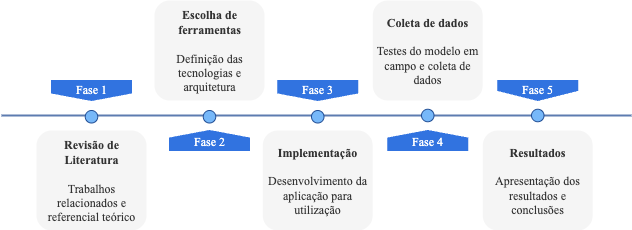
\includegraphics[width=\textwidth]{images/fases_pesquisa.png}
		\fonte{Elaborado pelo autor}
	\end{minipage}
\end{figure}
\FloatBarrier

\subsection{Proposta de Solução}

Atualmente, observa-se que o impacto da Inteligência Artificial no desenvolvimento de \textit{software} ainda é um tema em debate, sendo comum que as análises existentes se restrinjam a relatos de uso ou percepções subjetivas por parte dos desenvolvedores. Em muitos casos, a avaliação da influência da IA sobre fatores como produtividade e tempo de execução de tarefas ocorre de forma fragmentada, sem um método padronizado que permita mensurar de maneira objetiva os efeitos reais de tais ferramentas.

Dentro desse cenário, este estudo propõe a elaboração de um desafio técnico, disponibilizado por meio de uma plataforma \textit{web} desenvolvida especificamente para este fim. Essa plataforma funcionará como um ambiente de avaliação controlado, no qual os participantes serão previamente organizados em dois grupos: um grupo com autorização para utilizar ferramentas de IA durante a resolução do desafio e outro grupo que deverá realizar a atividade sem recorrer a tais recursos.

A proposta busca, assim, criar condições equivalentes para ambos os grupos, garantindo que todos recebam o mesmo enunciado do desafio, apresentado diretamente na plataforma. Para cada participante será disponibilizado um link único, correspondente ao grupo ao qual pertence. A partir desse acesso, o desenvolvedor poderá visualizar as instruções, iniciar a tarefa e, ao concluir, submeter os arquivos com sua solução.

A plataforma também atuará como mecanismo de registro, armazenando automaticamente o tempo total gasto por cada participante, desde o momento em que deu início ao desafio até a finalização da entrega. Dessa forma, além da coleta da solução proposta, será possível analisar métricas objetivas como tempo de conclusão, qualidade do código entregue e eventuais diferenças de abordagem entre os grupos.

\section{Modelo Proposto}

Esta seção tem como objetivo descrever brevemente a ferramenta desenvolvida e utilizada para a execução deste trabalho, incluindo sua arquitetura, funcionalidades e tecnologias utilizadas. O modelo proposto consiste em uma aplicação \textit{web} que centraliza as informações do desafio técnico, disponibilizando-o de forma prática e organizada para os desenvolvedores participantes do estudo.

A aplicação coleta o nome e o cargo atual do participante no mercado de trabalho. O nome é utilizado exclusivamente para exibir uma mensagem personalizada de boas-vindas. Funciona como um identificador simples durante a sessão, mantendo o usuário ativo no desafio, sem necessidade de cadastro, \textit{tokens} ou \textit{logins} complexos. Dessa forma, os nomes dos participantes não são utilizados na apresentação dos resultados do estudo, garantindo anonimato e simplicidade na utilização da ferramenta.

\subsection{Visão Geral}

Lorem ipsum.

\subsection{Arquitetura e Tecnologias}

Lorem ipsum.

\subsection{Funcionalidades}

Lorem ipsum.

\subsection{Formulário Inicial}

Lorem ipsum.

\subsection{Tela Inicial e Informações do Desafio}

Lorem ipsum.

\section{Análise e Discussão dos Resultados}

Lorem ipsum.

\subsection{Coleta de Dados}

Lorem ipsum.

\subsection{Avaliação dos Resultados}

Lorem ipsum.

\section{Considerações Finais e Trabalhos Futuros}

Lorem ipsum.

\bibliography{references}

\appendix
\section{DIAGRAMA ER DO BANCO DE DADOS}

Lorem ipsum.

\section{TELAS DA APLICAÇÃO}

Lorem ipsum.

\section{TEXTO TEXTO}

Lorem ipsum.

\section{CENÁRIOS DE TESTES}

Lorem ipsum.

\section{TEXTO TEXTO}

Lorem ipsum.

\section{TEXTO TEXTO}

Lorem ipsum.

\section{RESPOSTAS DO QUESTIONÁRIO}

Lorem ipsum.

\section{REQUISITOS FUNCIONAIS DA APLICAÇÃO}

Lorem ipsum.

\section{TEXTO TEXTO}

Lorem ipsum.

\annex
\section{NOME DO ANEXO}

Lorem ipsum.

\end{document}
